         \chapter{Electric circuits}
    \setcounter{figure}{1}
    \setcounter{subfigure}{1}
    \label{f13bac5321b85aca0e213ebdf4f72465}
         \section{ Introduction and key concepts}
    \nopagebreak
            \label{m38771} $ \hspace{-5pt}\begin{array}{cccccccccccc}   
\includegraphics[width=0.75cm]{col11305.imgs/summary_fullmarks.png} &   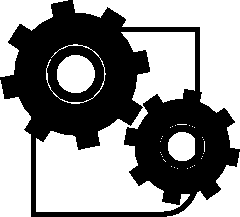
\includegraphics[width=0.75cm]{col11305.imgs/summary_simulation.png} &   \end{array} $ \hspace{2 pt}\raisebox{-5 pt}{} {(section shortcode: P10074 )} \par 
    \label{m38771*cid2}
            \subsection{ Electric Circuits}
            \nopagebreak
      \label{m38771*id62184}People all over the world depend on electricity to provide power for most appliances in the home and at work. For example, fluorescent lights, electric heating and cooking (on electric stoves), all depend on electricity to work.
To realise just how big an impact electricity has on our daily lives, just think about what happens when there is a power
failure or load shedding.\par 
\label{m38771*secfhsst!!!underscore!!!id72}
            \subsubsection{  Discussion : Uses of electricity }
            \nopagebreak
      \label{m38771*id62198}With a partner, take the following topics and, for each topic, write down at least 5 items/appliances/machines which need
electricity to work. Try not to use the same item more than once.\par 
      \label{m38771*id62544}\begin{itemize}[noitemsep]
            \label{m38771*uid1}\item At home
\label{m38771*uid2}\item At school
\label{m38771*uid3}\item At the hospital
\label{m38771*uid4}\item In the city
\end{itemize}
      \label{m38771*id62592}Once you have finished making your lists, compare with the lists of other people in your class. (Save your lists somewhere safe for later because there will be another activity for which you'll need them.)\par 
      \label{m38771*id62597}When you start comparing, you should notice that there are many different items which we use in our daily lives which rely on electricity to work!
 \par 
\label{m38771*notfhsst!!!underscore!!!id89}
\begin{tabular}{cc}
	   \hspace*{-50pt}\raisebox{-8 mm}{ 
\includegraphics[width=0.5in]{col11305.imgs/pstip2.png}  }& 
	\begin{minipage}{0.85\textwidth}
	\begin{note}
      {tip: }\textbf{Safety Warning:}
We believe in experimenting and learning about physics at every opportunity, BUT
playing with electricity and electrical appliances can be \textbf{EXTREMELY DANGEROUS}! Do not try to build
homemade circuits alone. Make sure you have someone with you who knows if what you are doing is safe.
Normal electrical outlets are dangerous. Treat electricity with respect in your everyday life. Do not touch exposed wires and do not approach downed power lines.
	\end{note}
	\end{minipage}
	\end{tabular}
	\par
      \label{m38771*uid5}
            \subsubsection{ Closed circuits}
            \nopagebreak
        \label{m38771*id62637}In the following activity we will investigate what is needed to cause charge to flow in an electric circuit.\par 
\label{m38771*secfhsst!!!underscore!!!id97}
            \subsubsection{ Experiment : Closed circuits }
            \nopagebreak
            \label{m38771*id62648}\noindent{}\textbf{Aim:}
To determine what is required to make electrical charges flow.
In this experiment, we will use a lightbulb to check whether electrical charge is flowing in the circuit or not. If charge is flowing, the lightbulb should glow. On the other hand, if no charge is flowing, the lightbulb will not glow.\par 
        \label{m38771*id62665}\noindent{}\textbf{Apparatus:}
        You will need a small lightbulb which is attached to a metal conductor (e.g. a bulb from a school electrical kit), some connecting wires and a battery.\par 
        \label{m38771*id62679}\noindent{}\textbf{Method:}
        Take the apparatus items and try to connect them in a way that you cause the light bulb to glow (i.e. charge flows in the circuit).\par 
        \label{m38771*id62694}\noindent{}\textbf{Questions:}
        \label{m38771*id62702}\begin{enumerate}[noitemsep, label=\textbf{\arabic*}. ] 
            \label{m38771*uid6}\item Once you have arranged your circuit elements to make the lightbulb glow, draw your circuit.
\label{m38771*uid7}\item What can you say about how the battery is connected? (i.e. does it have one or two connecting leads attached? Where are they attached?)
\label{m38771*uid8}\item What can you say about how the light bulb is connected in your circuit? (i.e. does it connect to one or two connecting leads, and where are they attached?)
\label{m38771*uid9}\item Are there any items in your circuit which are not attached to something? In other words, are there any gaps in your circuit?
\end{enumerate}
        \par 
        \label{m38771*id62757}Write down your conclusion about what is needed to make an electric circuit work and charge to flow.
 \par 
        \label{m38771*id62768}In the experiment above, you will have seen that the light bulb only glows when there is a \textsl{closed} circuit i.e. there are no gaps in the circuit and all the circuit elements are connected in a \textsl{closed loop}. Therefore, in order for charges to flow, a closed circuit and an energy source (in this case the battery) are needed. (Note: you do not have to have a lightbulb in the circuit! We used this as a check that charge was flowing.)\par 
\label{m38771*fhsst!!!underscore!!!id128}\begin{definition}
	  \begin{tabular*}{15 cm}{m{15 mm}m{}}
	\hspace*{-50pt}  
\includegraphics[width=0.5in]{col11305.imgs/psflag2.png}   & \Definition{   \label{id2477990}\textbf{ Electric circuit }} { \label{m38771*meaningfhsst!!!underscore!!!id128}
        \label{m38771*id62792}An electric circuit is a closed path (with no breaks or gaps) along which electrical charges (electrons) flow powered by an energy source. \par 
         } 
      \end{tabular*}
      \end{definition}
      \label{m38771*uid10}
            \subsubsection{ Representing electric circuits}
            \nopagebreak
        \label{m38771*uid11}
            \subsubsection{ Components of electrical circuits}
            \nopagebreak
          \label{m38771*id62821}Some common elements (components) which can be found in electrical circuits include light bulbs, batteries, connecting leads, switches, resistors, voltmeters and ammeters. You will learn more about these items in later sections, but it is important to know what their symbols are and how to represent them in circuit diagrams. Below is a table with the items and their symbols:\par 
    % \textbf{m38516*uid12}\par
          \begin{table}[H]
    % \begin{table}[H]
    % \\ '' '0'
        \begin{center}
      \label{m38773*id67892}
    \noindent
    \tabletail{%
        \hline
        \multicolumn{3}{|p{\mytableboxwidth}|}{\raggedleft \small \sl continued on next page}\\
        \hline
      }
      \tablelasttail{}
      \begin{xtabular}[t]{|l|l|l|}\hline
                  \textbf{Instrument}
                 &
                  \textbf{Measured Quantity}
                 &
                  \textbf{Proper Connection}
                % make-rowspan-placeholders
     \tabularnewline\cline{1-1}\cline{2-2}\cline{3-3}
      %--------------------------------------------------------------------
        Voltmeter &
        Voltage &
        In Parallel% make-rowspan-placeholders
     \tabularnewline\cline{1-1}\cline{2-2}\cline{3-3}
      %--------------------------------------------------------------------
        Ammeter &
        Current &
        In Series% make-rowspan-placeholders
     \tabularnewline\cline{1-1}\cline{2-2}\cline{3-3}
      %--------------------------------------------------------------------
    \end{xtabular}
      \end{center}
    \begin{center}{\small\bfseries Table 16.2}\end{center}
    \begin{caption}{\small\bfseries Table 16.2}\end{caption}
\end{table}
    \par
  \label{m38773**end}
         \section{ Resistance}
    \nopagebreak
            \label{m38776} $ \hspace{-5pt}\begin{array}{cccccccccccc}   
\includegraphics[width=0.75cm]{col11305.imgs/summary_fullmarks.png} &   
\includegraphics[width=0.75cm]{col11305.imgs/summary_video.png} &   \end{array} $ \hspace{2 pt}\raisebox{-5 pt}{} {(section shortcode: P10077 )} \par 
    \label{m38776*cid5}
            \subsection{ Resistance}
            \nopagebreak
      \label{m38776*sb1235}
	The resistance of a circuit element can be thought of as how much it opposes the flow of electric current in the circuit. 
	\vspace{\rubberspace}\par
        \label{m38776*fhsst!!!underscore!!!id1729}\begin{definition}
	  \begin{tabular*}{15 cm}{m{15 mm}m{}}
	\hspace*{-50pt}  
\includegraphics[width=0.5in]{col11305.imgs/psflag2.png}   & \Definition{   \label{id2485077}\textbf{ Resistance }} { \label{m38776*meaningfhsst!!!underscore!!!id1729}
        \label{m38776*id67260} The resistance of a conductor is defined as the potential difference across it divided by the current flowing though it. We use the symbol \textbf{R} to show resistance and it is measured in units called \textbf{Ohms} with the symbol $\mathrm{\Omega }$.\par 
        \label{m38776*id67288}\nopagebreak\noindent{}
          
    \begin{equation}
    1\phantom{\rule{4pt}{0ex}}\mathrm{Ohm}=1\frac{\mathrm{Volt}}{\mathrm{Ampere}}.\tag{16.30}
      \end{equation}
         } 
      \end{tabular*}
      \end{definition}
	\par 
      \label{m38776*uid62}
            \subsubsection{ What causes resistance?}
            \nopagebreak
        \label{m38776*id67246}We have spoken about resistors that reduce the flow of charge
in a conductor. On a microscopic level, electrons moving through
the conductor collide with the particles of which the conductor
(metal) is made. When they collide, they transfer kinetic energy.
The electrons lose kinetic energy and slow down. This leads to
resistance. The transferred energy causes the resistor to heat up.
You can feel this directly if you touch a cellphone charger when you are charging a cell phone - the charger gets warm because its circuits have some resistors in them!\par 
        \label{m38776*id67330}\textsl{All} conductors have some resistance. For example, a piece of wire
has less resistance than a light bulb, but both have resistance. A lightbulb is a very thin wire surrounded by a glass housing The high resistance of the filament (small wire) in a lightbulb causes the electrons to
transfer a lot of their kinetic energy in the form of heat\label{m38776*uid63}\footnote{Flourescent lightbulbs do not use thin wires; they use the fact that certain gases glow when a current flows through them. They are much more efficient (much less resistance) than lightbulbs.}. The heat energy is enough
to cause the filament to glow white-hot which produces light. The wires
connecting the lamp to the cell or battery hardly even get warm while
conducting the same amount of current. This is because of their
much lower resistance due to their larger cross-section (they are thicker).\par 
        \label{m38776*id67354}An important effect of a resistor is that it \textsl{converts} electrical
energy into \textbf{heat} energy. \textbf{Light} is a by-product of the heat that is produced.\par 
\label{m38776*notfhsst!!!underscore!!!id1758}
\begin{tabular}{cc}
	\hspace*{-50pt}\raisebox{-8 mm}{\hspace{-0.2in}
\includegraphics[width=0.75in]{col11305.imgs/psfact2.png} } & 
	\begin{minipage}{0.85\textwidth}
	\begin{note}
      {note: } There is a special type of conductor,
called a \textbf{superconductor} that has no resistance, but the
materials that make up all known superconductors only start superconducting
at very low temperatures (approximately -170${}^{\circ }$C).
	\end{note}
	\end{minipage}
	\end{tabular}
	\par
 \label{m38776*uid64}
            \subsubsection{ Why do batteries go flat?}
            \nopagebreak
          \label{m38776*id67413}A battery stores chemical potential energy. When it is connected in a circuit, a chemical reaction takes place inside the battery which converts chemical potential energy to electrical energy which powers the charges (electrons) to move through the circuit. All the circuit elements (such as the conducting leads, resistors and lightbulbs) have some resistance to the flow of charge and convert the electrical energy to heat and, in the case of the lightbulb, heat and light.
Since energy is always conserved, the battery goes flat when all its chemical potential energy has been converted into other forms of energy.\par 
      \label{m38776*uid65}
            \subsubsection{ Resistors in electric circuits}
            \nopagebreak
        \label{m38776*id67431}It is important to understand what effect adding resistors to a circuit has on the \textsl{total} resistance of a circuit and on the current that can flow in the circuit.\par 
        \label{m38776*uid66}
            \subsubsection{ Resistors in series}
            \nopagebreak
          \label{m38776*id67450}When we add resistors in series to a circuit, we \textsl{increase} the resistance to the flow of current. There is only \textbf{one path} along which the current can flow and the current is the same at all places in the series circuit. Take a look at the diagram below: On the left there is a circuit with a single resistor and a battery. No matter where we measure the current, it is the same in a series circuit. On the right, we have added a second resistor in series to the circuit. The \textsl{total} resistance of the circuit has \textsl{increased} and you can see from the reading on the ammeter that the current in the circuit has \textsl{decreased} and is still the same everywhere in the circuit.\par 
          \label{m38776*id67481}
    \setcounter{subfigure}{0}
	\begin{figure}[H] % horizontal\label{m38776*id67485}
    \begin{center}
    \label{m38776*id67485!!!underscore!!!media}\label{m38776*id67485!!!underscore!!!printimage}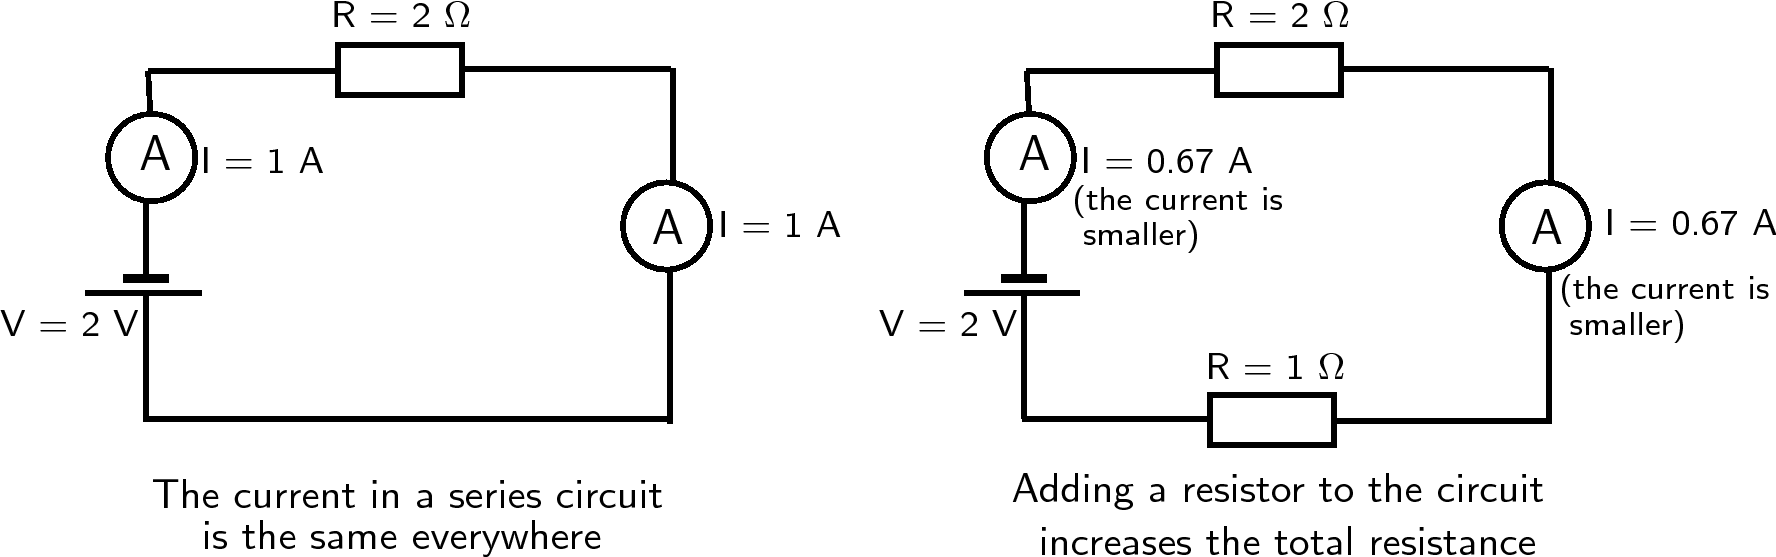
\includegraphics{col11305.imgs/m38776_PG10C9_032.png} % m38776;PG10C9\_032.png;;;6.0;8.5;
      \vspace{2pt}
    \vspace{.1in}
    \end{center}
 \end{figure}       
          \par 
\label{m38776*id64070}\noindent{}\textbf{Potential difference and resistors in series}When resistors are in series, one after the other, there is a potential difference across each resistor. The total potential difference across a set of resistors in series is the sum of the potential differences across each of the resistors in the set. This is the same as falling a large distance under gravity or falling that same distance (difference) in many smaller steps. The total distance (difference) is the same.\par 
        \label{m38776*id64076}Look at the circuits below. If we measured the potential difference between the black dots in all of these circuits it would be the same; it is just the potential difference across the battery which is the same as the potential difference across the rest of the circuit. So we now know the total potential difference is the same across one, two or three resistors. We also know that some work is required to make charge flow through each one. Each is a step down in potential energy. These steps add up to the total voltage drop which we know is the difference between the two dots.
The sum of the potential differences across each individual resistor is equal to the potential difference measured across all of them together. For this reason, series circuits are sometimes called \textbf{voltage dividers}.\par 
        \label{m38776*id64084}
    \setcounter{subfigure}{0}
	\begin{figure}[H] % horizontal\label{m38776*id64087}
    \begin{center}
    \label{m38776*id64087!!!underscore!!!media}\label{m38776*id64087!!!underscore!!!printimage}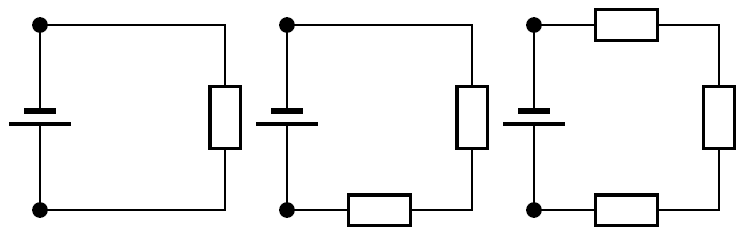
\includegraphics[width=\columnwidth]{col11305.imgs/m38776_PG10C9_018.png} % m38776;PG10C9\_018.png;;;6.0;8.5;
      \vspace{2pt}
    \vspace{.1in}
    \end{center}
 \end{figure}       
        \par 
        \label{m38776*id64094}Let us look at this in a bit more detail. In the picture below you can see what the different measurements for 3 identical resistors in series could look like. The total voltage across all three resistors is the sum of the voltages across the individual resistors. \par 
        \label{m38776*id64099}
    \setcounter{subfigure}{0}
	\begin{figure}[H] % horizontal\label{m38776*id64102}
    \begin{center}
    \label{m38776*id64102!!!underscore!!!media}\label{m38776*id64102!!!underscore!!!printimage}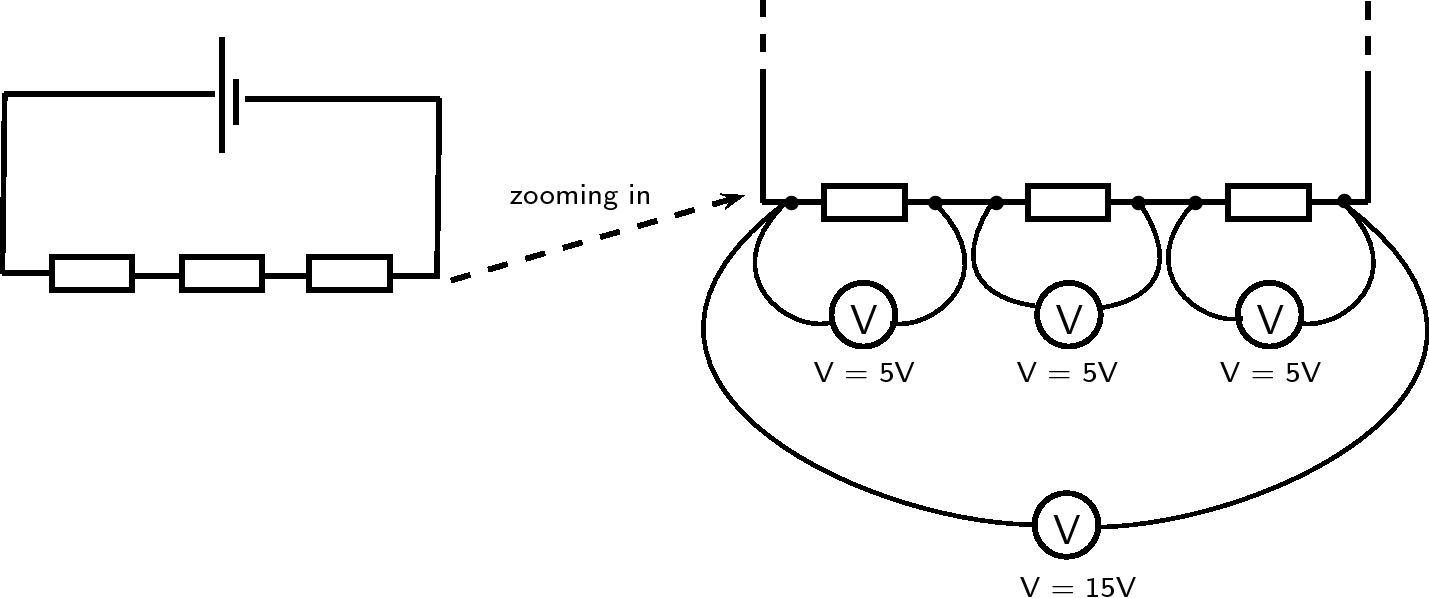
\includegraphics{col11305.imgs/m38776_PG10C9_019.png} % m38776;PG10C9\_019.png;;;6.0;8.5;
      \vspace{2pt}
    \vspace{.1in}
    \end{center}
 \end{figure}       
        \par 
\label{m38776*uid25342}
            \subsubsection{ Equivalent Series Resistance}
            \nopagebreak
            \label{m38776*id63926}When there is more than one resistor in a circuit, we are usually able to calculate the total combined resitance of all the resistors. The resistance of the single resistor is known as \textsl{equivalent resistance} or total resistance.
Consider a circuit consisting of three resistors and a single cell connected in series.\par 
          \label{m38776*id63930}
    \setcounter{subfigure}{0}
	\begin{figure}[H] % horizontal\label{m38776*id63934}
    \begin{center}
    \label{m38776*id63934!!!underscore!!!media}\label{m38776*id63934!!!underscore!!!printimage}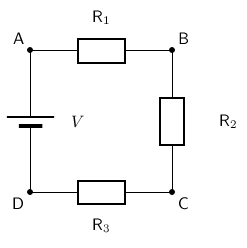
\includegraphics[width=0.4\columnwidth]{col11305.imgs/m38776_PG11C9_007.png} % m38776;PG11C9\_007.png;;;6.0;8.5;
      \vspace{2pt}
    \vspace{.1in}
    \end{center}
 \end{figure}       
          \par 
\label{m38776*eip-546}We can define the total resistance in a series circuit as:\par \label{m38776*fhsst!!!underscore!!!id788}\begin{definition}
	  \begin{tabular*}{15 cm}{m{15 mm}m{}}
	\hspace*{-50pt}  
\includegraphics[width=0.5in]{col11305.imgs/psflag2.png}   & \Definition{   \label{id2485652}\textbf{ Equivalent resistance in a series circuit, ${R}_{s}$ }} { \label{m38776*meaningfhsst!!!underscore!!!id788}
          \label{m38776*id64628}For $n$ resistors in series the equivalent resistance is:\par 
          \label{m38776*uid2532}\nopagebreak\noindent{}
            
    \begin{equation}
    {R}_{s}={R}_{1}+{R}_{2}+{R}_{3}+\cdots +{R}_{n}\tag{16.31}
      \end{equation}
           } 
      \end{tabular*}
      \end{definition}
          \label{m38776*id64719}The more resistors we add in series, the higher the equivalent resistance in the circuit. Since the resistors act as obstacles to the flow of charge through the circuit, the current in the circuit is reduced. Therefore, the \textsl{higher} the resistance in the circuit, the \textsl{lower} the current through the battery and the circuit. We say that the current in the battery is inversely proportional to the resistance in the circuit. 
Let us apply the rule of equivalent resistance in a series circuit to the following circuit.\par 
          \label{m38776*id64722}
    \setcounter{subfigure}{0}
	\begin{figure}[H] % horizontal\label{m38776*id64726}
    \begin{center}
    \label{m38776*id64726!!!underscore!!!media}\label{m38776*id64726!!!underscore!!!printimage}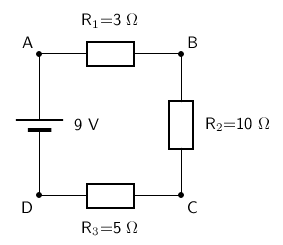
\includegraphics[width=0.4\columnwidth]{col11305.imgs/m38776_PG11C9_008.png} % m38776;PG11C9\_008.png;;;6.0;8.5;
      \vspace{2pt}
    \vspace{.1in}
    \end{center}
 \end{figure}       
          \par 
          \label{m38776*id64732}The resistors are in series, therefore:\par 
          \label{m38776*id64736}\nopagebreak\noindent{}
    \begin{equation}
    \begin{array}{ccc}\hfill {R}_{s}& =& {R}_{1}+{R}_{2}+{R}_{3}\hfill \\ & =& 3\phantom{\rule{0.166667em}{0ex}}\mathrm{\Omega }+10\phantom{\rule{0.166667em}{0ex}}\mathrm{\Omega }+5\phantom{\rule{0.166667em}{0ex}}\mathrm{\Omega }\hfill \\ & =& 18\phantom{\rule{0.166667em}{0ex}}\mathrm{\Omega }\hfill \end{array}\tag{16.32}
      \end{equation}
\label{m38776*eip-186}
            \subsubsection{ Experiment : Current in Series Circuits}
            \nopagebreak
            \label{m38776*id66871}\noindent{}\textbf{Aim:}
          To determine the effect of multiple resistors on current in a circuit\par 
        \label{m38776*id66886}\noindent{}\textbf{Apparatus:}
        \label{m38776*id66895}\begin{itemize}[noitemsep]
            \label{m38776*uid49}\item Battery
\label{m38776*uid50}\item Resistors
\label{m38776*uid51}\item Light bulb
\label{m38776*uid52}\item Wires
\end{itemize}
        \par 
        \label{m38776*id66948}\noindent{}\textbf{Method:}
        \label{m38776*id66957}\begin{enumerate}[noitemsep, label=\textbf{\arabic*}. ] 
            \label{m38776*uid53}\item Construct the following circuits
    \setcounter{subfigure}{0}
	\begin{figure}[H] % horizontal\label{m38776*id66976}
    \begin{center}
    \label{m38776*id66976!!!underscore!!!media}\label{m38776*id66976!!!underscore!!!printimage}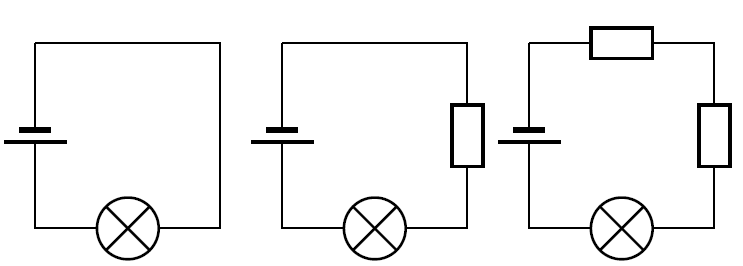
\includegraphics[width=\columnwidth]{col11305.imgs/m38776_PG10C9_027.png} % m38776;PG10C9\_027.png;;;6.0;8.5;
      \vspace{2pt}
    \vspace{.1in}
    \end{center}
 \end{figure}       \label{m38776*uid54}\item Rank the three circuits in terms of the brightness of the bulb.
\end{enumerate}
        \par 
        \label{m38776*id66996}\noindent{}\textbf{Conclusions:}
        The brightness of the bulb is an indicator of how much current is flowing. If the bulb gets brighter because of a change then more current is flowing. If the bulb gets dimmer less current is flowing.
You will find that the more resistors you have the dimmer the bulb.
 \par 
\label{m38776*secfhsst!!!underscore!!!id903}\vspace{.5cm} 
      \noindent
      \hspace*{-30pt}
\includegraphics[width=0.5in]{col11305.imgs/pspencil2.png}   \raisebox{25mm}{   
      \begin{mdframed}[linewidth=4, leftmargin=40, rightmargin=40]  
      \begin{exercise}
    \noindent\textbf{Exercise 16.11:  Equivalent series resistance I }
          \label{m38776*probfhsst!!!underscore!!!id904}
          \label{m38776*id64862}Two 10 k$\Omega $ resistors are connected in series. Calculate the equivalent resistance. \par 
          \vspace{5pt}
          \label{m38776*solfhsst!!!underscore!!!id907}\noindent\textbf{Solution to Exercise } \label{m38776*listfhsst!!!underscore!!!id907}\begin{enumerate}[noitemsep, label=\textbf{Step} \textbf{\arabic*}. ] 
            \leftskip=20pt\rightskip=\leftskip\item  
          \label{m38776*id64896}Since the resistors are in series we can use:\par 
          \label{m38776*id64899}\nopagebreak\noindent{}
            
    \begin{equation}
    {R}_{s}={R}_{1}+{R}_{2}\tag{16.33}
      \end{equation}
          \item  
          \label{m38776*id64940}\nopagebreak\noindent{}
            
    \begin{equation}
    \begin{array}{ccc}\hfill {R}_{s}& =& {R}_{1}+{R}_{2}\hfill \\ & =& 10\phantom{\rule{0.166667em}{0ex}}\mathrm{k}\phantom{\rule{0.166667em}{0ex}}\Omega +10\phantom{\rule{0.166667em}{0ex}}\mathrm{k}\phantom{\rule{0.166667em}{0ex}}\Omega \hfill \\ & =& 20\phantom{\rule{0.166667em}{0ex}}\mathrm{k}\phantom{\rule{0.166667em}{0ex}}\Omega \hfill \end{array}\tag{16.34}
      \end{equation}
          \item  
          \label{m38776*id65061}The equivalent resistance of two 10 k$\Omega $ resistors connected in series is 20 k$\Omega $. \par 
          \end{enumerate}
    \end{exercise}
    \end{mdframed}
    }
    \noindent
\label{m38776*secfhsst!!!underscore!!!id1001}\vspace{.5cm} 
      \noindent
      \hspace*{-30pt}
\includegraphics[width=0.5in]{col11305.imgs/pspencil2.png}   \raisebox{25mm}{   
      \begin{mdframed}[linewidth=4, leftmargin=40, rightmargin=40]  
      \begin{exercise}
    \noindent\textbf{Exercise 16.12:  Equivalent series resistance II }
          \label{m38776*probfhsst!!!underscore!!!id1002}
          \label{m38776*id65108}Two resistors are connected in series. The equivalent resistance is 100 $\Omega $. If one resistor is 10 $\Omega $, calculate the value of the second resistor. \par 
          \vspace{5pt}
          \label{m38776*solfhsst!!!underscore!!!id1005}\noindent\textbf{Solution to Exercise } \label{m38776*listfhsst!!!underscore!!!id1005}\begin{enumerate}[noitemsep, label=\textbf{Step} \textbf{\arabic*}. ] 
            \leftskip=20pt\rightskip=\leftskip\item  
          \label{m38776*id65152}Since the resistors are in series we can use:\par 
          \label{m38776*id65155}\nopagebreak\noindent{}
            
    \begin{equation}
    {R}_{s}={R}_{1}+{R}_{2}\tag{16.35}
      \end{equation}
          \label{m38776*id65192}We are given the value of ${R}_{s}$ and ${R}_{1}$.\par 
          \item  
          \label{m38776*id65230}\nopagebreak\noindent{}
            
    \begin{equation}
    \begin{array}{ccc}\hfill {R}_{s}& =& {R}_{1}+{R}_{2}\hfill \\ \hfill \therefore {R}_{2}& =& {R}_{s}-{R}_{1}\hfill \\ & =& 100\phantom{\rule{0.166667em}{0ex}}\Omega -10\phantom{\rule{0.166667em}{0ex}}\Omega \hfill \\ & =& 90\phantom{\rule{0.166667em}{0ex}}\Omega \hfill \end{array}\tag{16.36}
      \end{equation}
          \item  
          \label{m38776*id65371}The second resistor has a resistance of 90 $\Omega $. \par 
          \end{enumerate}
    \end{exercise}
    \end{mdframed}
    }
    \noindent
    \setcounter{subfigure}{0}
	\begin{figure}[H] % horizontal\label{m38776*circuits-2}
    \textnormal{Khan academy video on circuits - 2}\vspace{.1in} \nopagebreak
  \label{m38776*yt-media2}\label{m38776*yt-video2}
            \raisebox{-5 pt}{ 
\includegraphics[width=0.5cm]{col11305.imgs/summary_www.png}} { (Video:  P10078 )}
      \vspace{2pt}
    \vspace{.1in}
 \end{figure}       
        \label{m38776*uid67}
            \subsubsection{ Resistors in parallel}
            \nopagebreak
          \label{m38776*id67501}In contrast to the series case, when we add resistors in parallel, we create \textbf{more paths} along which current can flow. By doing this we \textsl{decrease} the total resistance of the circuit!\par 
          \label{m38776*id67518}Take a look at the diagram below. On the left we have the same circuit as shown on the left in Figure~16.25 with a battery and a resistor. The ammeter shows a current of 1 ampere. On the right we have added a second resistor in parallel to the first resistor. This has increased the number of paths (branches) the charge can take through the circuit - the total resistance has decreased. You can see that the current in the circuit has increased. Also notice that the current in the different branches can be different (in this case 1 A and 2 A) but must add up to the current through the battery (3 A). Since the total current in the circuit is equal to the sum of the currents in the parallel branches, a parallel circuit is sometimes called a \textbf{current divider}.\par 
          \label{m38776*id67525}
    \setcounter{subfigure}{0}
	\begin{figure}[H] % horizontal\label{m38776*id67528}
    \begin{center}
    \label{m38776*id67528!!!underscore!!!media}\label{m38776*id67528!!!underscore!!!printimage}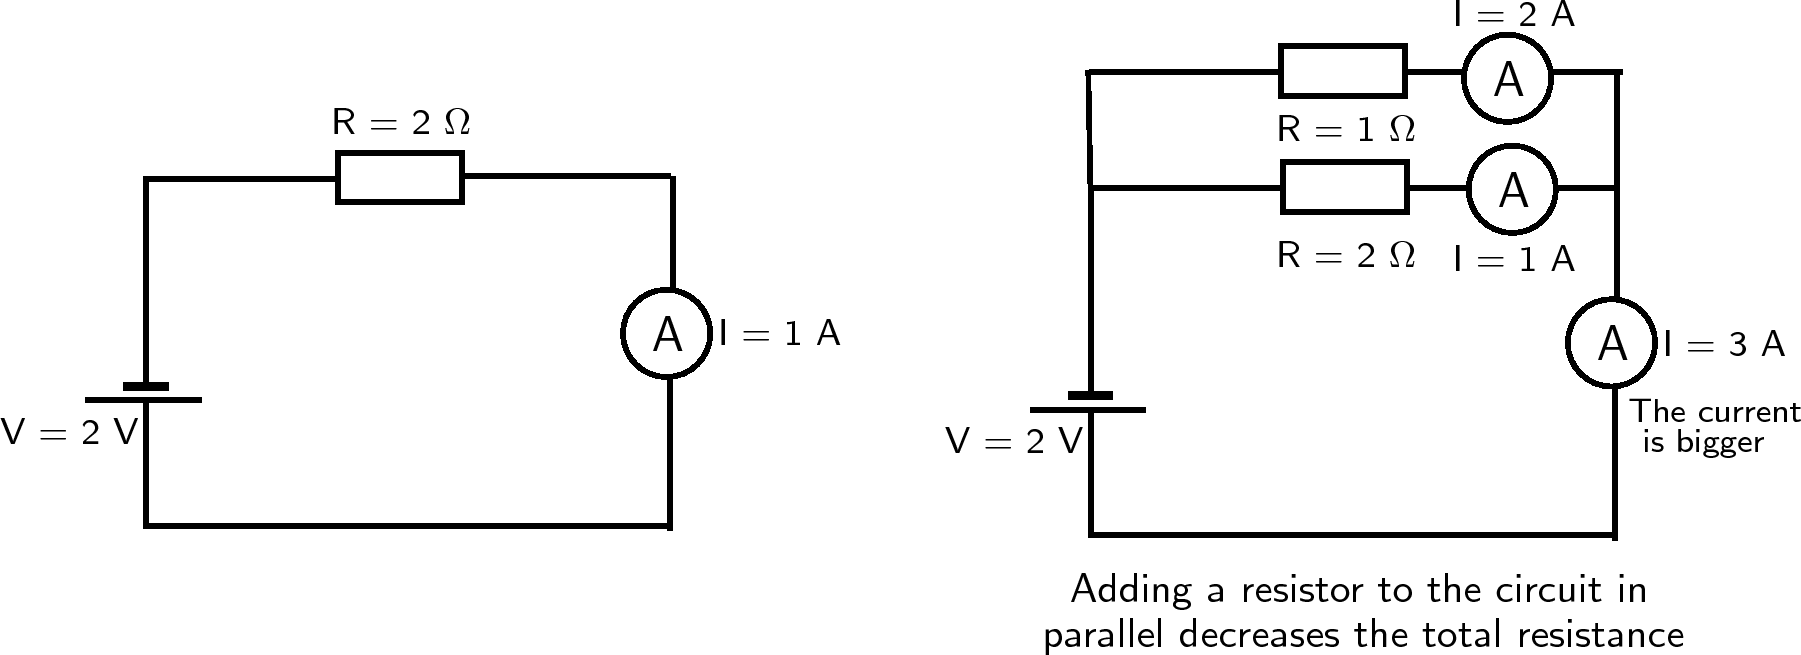
\includegraphics{col11305.imgs/m38776_PG10C9_033.png} % m38776;PG10C9\_033.png;;;6.0;8.5;
      \vspace{2pt}
    \vspace{.1in}
    \end{center}
 \end{figure}       
          \par 
        \label{m38776*id64009}\noindent{}\textbf{Potential difference and parallel resistors}When resistors are connected in parallel the start and end points for all the resistors are the same. These points have the same potential energy and so the potential difference between them is the same no matter what is put in between them. You can have one, two or many resistors between the two points, the potential difference will not change. You can ignore whatever components are between two points in a circuit when calculating the difference between the two points.\par 
        \label{m38776*id64017}Look at the following circuit diagrams. The battery is the same in all cases. All that changes is that more resistors are added between the points marked by the black dots. If we were to measure the potential difference between the two dots in these circuits we would get the same answer for all three cases.\par 
        \label{m38776*id64023}
    \setcounter{subfigure}{0}
	\begin{figure}[H] % horizontal\label{m38776*id64026}
    \begin{center}
    \label{m38776*id64026!!!underscore!!!media}\label{m38776*id64026!!!underscore!!!printimage}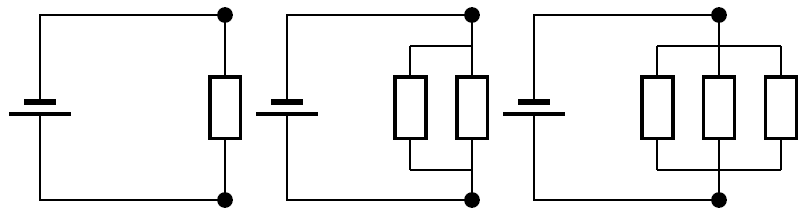
\includegraphics[width=\columnwidth]{col11305.imgs/m38776_PG10C9_016.png} % m38776;PG10C9\_016.png;;;6.0;8.5;
      \vspace{2pt}
    \vspace{.1in}
    \end{center}
 \end{figure}       
        \par 
        \label{m38776*id64033}Let's look at two resistors in parallel more closely. When you construct a circuit you use wires and you might think that measuring the voltage in different places on the wires will make a difference. This is not true. The potential difference or voltage measurement will only be different if you measure a different set of components. All points on the wires that have no circuit components between them will give you the same measurements.\par 
        \label{m38776*id64040}All three of the measurements shown in the picture below (i.e. A--B, C--D and E--F) will give you the same voltage. The different measurement points on the left (i.e. A, E, C) have no components between them so there is no change in potential energy.
Exactly the same applies to the different points on the right (i.e. B, F, D). When you measure the potential difference between the points on the left and right you will get the same answer.\par 
        \label{m38776*id64049}
    \setcounter{subfigure}{0}
	\begin{figure}[H] % horizontal\label{m38776*id64052}
    \begin{center}
    \label{m38776*id64052!!!underscore!!!media}\label{m38776*id64052!!!underscore!!!printimage}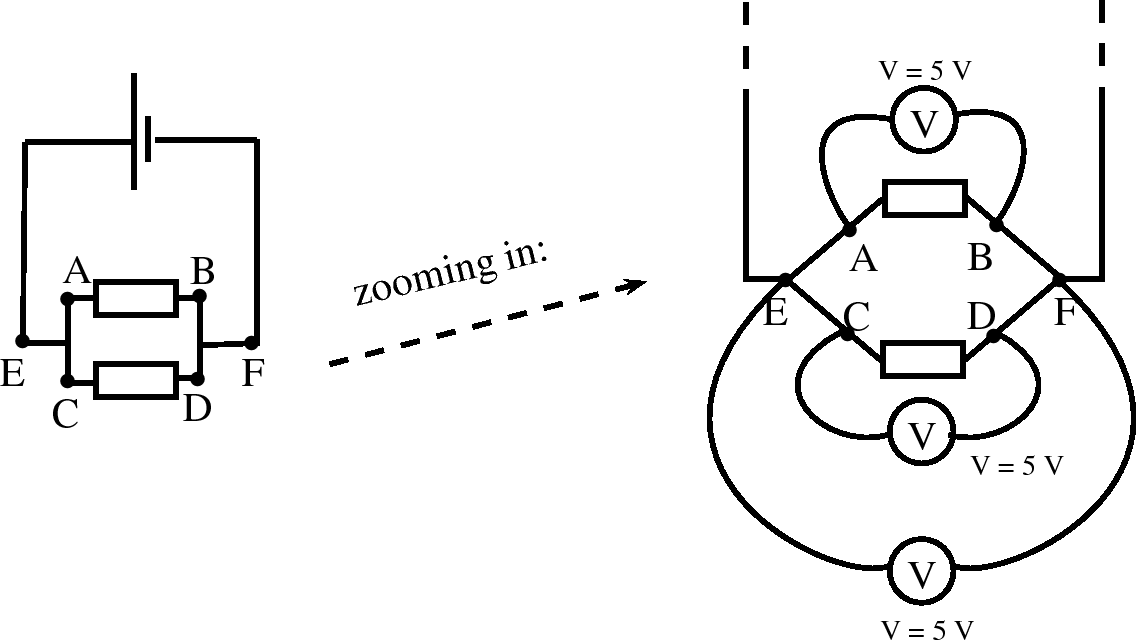
\includegraphics{col11305.imgs/m38776_PG10C9_017.png} % m38776;PG10C9\_017.png;;;6.0;8.5;
      \vspace{2pt}
    \vspace{.1in}
    \end{center}
 \end{figure}       
        \par 
        \label{m38776*eip-684}\label{m38776*eip-id1170813612376}\begin{definition}
	  \begin{tabular*}{15 cm}{m{15 mm}m{}}
	\hspace*{-50pt}  
\includegraphics[width=0.5in]{col11305.imgs/psflag2.png}   & \Definition{   \label{id2487246}\textbf{ Equivalent resistance of two parallel resistor, ${R}_{p}$ }} { \label{m38776*eip-id1170826978594}
          \label{m38776*eip-id1170816625786}For $2$ resistors in parallel with resistances ${R}_{1}$ and ${R}_{2}$, the equivalent resistance is:\par 
          \label{m38776*eip-id1170814512227}\nopagebreak\noindent{}
    \begin{equation}
    {R}_{p}=\frac{{R}_{1}{R}_{2}}{{R}_{1}+{R}_{2}}\tag{16.37}
      \end{equation}
           } 
      \end{tabular*}
      \end{definition}
\par \label{m38776*uid2446}
            \subsubsection{ Equivalent parallel resistance}
            \nopagebreak
            \label{m38776*id65406}Consider a circuit consisting of a single cell and three resistors that are connected in parallel.\par 
          \label{m38776*id65410}
    \setcounter{subfigure}{0}
	\begin{figure}[H] % horizontal\label{m38776*id65414}
    \begin{center}
    \label{m38776*id65414!!!underscore!!!media}\label{m38776*id65414!!!underscore!!!printimage}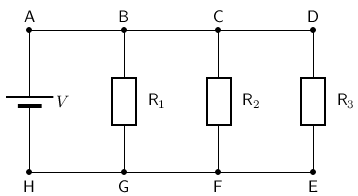
\includegraphics[width=300px]{col11305.imgs/m38776_PG11C9_009.png} % m38776;PG11C9\_009.png;;;6.0;8.5;
      \vspace{2pt}
    \vspace{.1in}
    \end{center}
 \end{figure}       
          \par 
\label{m38776*eip-754}Using what we know about voltage and current in parallel circuits we can define the equivalent resistance of several resistors in parallel as:\par \label{m38776*fhsst!!!underscore!!!id1576}\begin{definition}
	  \begin{tabular*}{15 cm}{m{15 mm}m{}}
	\hspace*{-50pt}  
\includegraphics[width=0.5in]{col11305.imgs/psflag2.png}   & \Definition{   \label{id2487427}\textbf{ Equivalent resistance in a parallel circuit, ${R}_{p}$ }} { \label{m38776*meaningfhsst!!!underscore!!!id1576}
          \label{m38776*id6613206}For $n$ resistors in parallel, the equivalent resistance is:\par 
          \label{m38776*uid2944}\nopagebreak\noindent{}
            
    \begin{equation}
    \frac{1}{{R}_{p}}=\left(\frac{1}{{R}_{1}}+\frac{1}{{R}_{2}}+\frac{1}{{R}_{3}}+\cdots +\frac{1}{{R}_{n}}\right)\tag{16.38}
      \end{equation}
           } 
      \end{tabular*}
      \end{definition}
          \label{m38776*id66324}Let us apply this formula to the following circuit.\par 
          \label{m38776*id66328}
    \setcounter{subfigure}{0}
	\begin{figure}[H] % horizontal\label{m38776*id66331}
    \begin{center}
    \label{m38776*id66331!!!underscore!!!media}\label{m38776*id66331!!!underscore!!!printimage}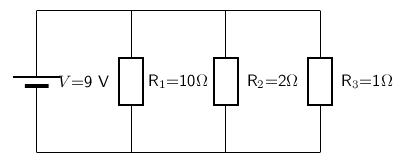
\includegraphics[width=300px]{col11305.imgs/m38776_PG11C9_010.png} % m38776;PG11C9\_010.png;;;6.0;8.5;
      \vspace{2pt}
    \vspace{.1in}
    \end{center}
 \end{figure}       
          \par 
          \label{m38776*id663318}What is the total resistance in the circuit?\par 
          \label{m38776*id66342}\nopagebreak\noindent{}
            
    \begin{equation}
    \begin{array}{ccc}\hfill \frac{1}{{R}_{p}}& =& \left(\frac{1}{{R}_{1}}+\frac{1}{{R}_{2}}+\frac{1}{{R}_{3}}\right)\hfill \\ & =& \left(\frac{1}{10\phantom{\rule{0.166667em}{0ex}}\Omega }+\frac{1}{2\phantom{\rule{0.166667em}{0ex}}\Omega }+\frac{1}{1\phantom{\rule{0.166667em}{0ex}}\Omega }\right)\hfill \\ & =& \left(\frac{1+5+10}{10}\right)\hfill \\ & =& \left(\frac{16}{10}\right)\hfill \\ \hfill \therefore {R}_{p}& =& 0,625\phantom{\rule{0.166667em}{0ex}}\Omega \hfill \end{array}\tag{16.39}
      \end{equation}
          \label{m38776*eip-234}
            \subsubsection{ Experiment : Current in Parallel Circuits }
            \nopagebreak
            \label{m38776*id67061}\noindent{}\textbf{Aim:}
          To determine the effect of multiple resistors on current in a circuit\par 
        \label{m38776*id67076}\noindent{}\textbf{Apparatus:}
        \label{m38776*id67085}\begin{itemize}[noitemsep]
            \label{m38776*uid56}\item Battery
\label{m38776*uid57}\item Resistors
\label{m38776*uid58}\item Light bulb
\label{m38776*uid59}\item Wires
\end{itemize}
        \par 
        \label{m38776*id67138}\noindent{}\textbf{Method:}
        \label{m38776*id67147}\begin{enumerate}[noitemsep, label=\textbf{\arabic*}. ] 
            \label{m38776*uid60}\item Construct the following circuits
    \setcounter{subfigure}{0}
	\begin{figure}[H] % horizontal\label{m38776*id67166}
    \begin{center}
    \label{m38776*id67166!!!underscore!!!media}\label{m38776*id67166!!!underscore!!!printimage}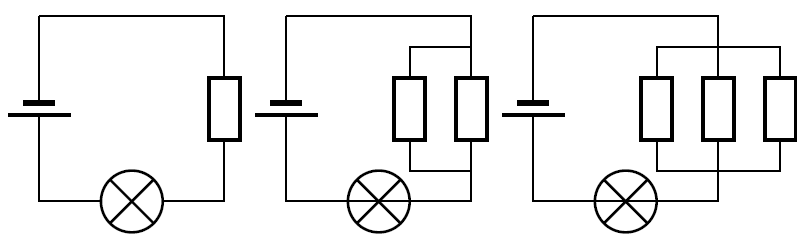
\includegraphics[width=\columnwidth]{col11305.imgs/m38776_PG10C9_030.png} % m38776;PG10C9\_030.png;;;6.0;8.5;
      \vspace{2pt}
    \vspace{.1in}
    \end{center}
 \end{figure}       \label{m38776*uid61}\item Rank the three circuits in terms of the brightness of the bulb.
\end{enumerate}
        \par 
        \label{m38776*id67186}\noindent{}\textbf{Conclusions:}
        The brightness of the bulb is an indicator of how much current is flowing. If the bulb gets brighter because of a change then more current is flowing. If the bulb gets dimmer less current is flowing.
You will find that the more resistors you have the brighter the bulb.
 \par \label{m38776*eip-828}Why is this the case? Why do more resistors make it easier for charge to flow in the circuit? It is because they are in parallel so there are more paths for charge to take to move. You can think of it like a highway with more lanes, or the tube of marbles splitting into multiple parallel tubes. The more branches there are, the easier it is for charge to flow. You will learn more about the total resistance of parallel resistors later but always remember that more resistors in parallel mean more pathways. In series the pathways come one after the other so it does not make it easier for charge to flow.\par \label{m38776*eip-291}\vspace{3.5cm} 
\vspace{\rubberspace}      
\hspace*{-30pt}
\includegraphics[width=0.5in]{col11305.imgs/pspencil2.png}   \raisebox{25mm}{   
      \begin{mdframed}[linewidth=4, leftmargin=40, rightmargin=40]  
      \begin{exercise}
    \noindent\textbf{Exercise 16.13}\label{m38776*probfhsst!!!underscore!!!id9084}
          \label{m38776*id648622}Two $8\phantom{\rule{2pt}{0ex}}\mathrm{k}\Omega $ resistors are connected in parallel. Calculate the equivalent resistance. \par 
          \vspace{5pt}
          \label{m38776*solfhsst!!!underscore!!!id9073}\noindent\textbf{Solution to Exercise } \label{m38776*listfhsst!!!underscore!!!id9074}\begin{enumerate}[noitemsep, label=\textbf{Step} \textbf{\arabic*}. ] 
            \leftskip=20pt\rightskip=\leftskip\item  
          \label{m38776*id648926}Since the resistors are in parallel we can use:\par 
          \label{m38776*id64849}\nopagebreak\noindent{}
            
    \begin{equation}
    \frac{1}{{R}_{p}}=\frac{1}{{R}_{1}}+\frac{1}{{R}_{2}}\tag{16.40}
      \end{equation}
          \item  
          \label{m38776*id6494034}\nopagebreak\noindent{}
            
    \begin{equation}
    \begin{array}{ccc}\hfill \frac{1}{{R}_{p}}& =& \frac{1}{{R}_{1}}+\frac{1}{{R}_{2}}\hfill \\ & =& \frac{1}{8\phantom{\rule{0.166667em}{0ex}}\mathrm{k}\phantom{\rule{0.166667em}{0ex}}\Omega }+\frac{1}{10\phantom{\rule{0.166667em}{0ex}}\mathrm{k}\phantom{\rule{0.166667em}{0ex}}\Omega }\hfill \\ \hfill {R}_{p}& =& \frac{2}{8}\hfill \\ & =& 4\phantom{\rule{0.166667em}{0ex}}\mathrm{k}\phantom{\rule{0.166667em}{0ex}}\Omega \hfill \end{array}\tag{16.41}
      \end{equation}
          \item  
          \label{m38776*id650261}The equivalent resistance of two $8\phantom{\rule{2pt}{0ex}}\mathrm{k}\Omega $ resistors connected in parallel is $4\phantom{\rule{2pt}{0ex}}\mathrm{k}\Omega $. \par 
          \end{enumerate}
    \end{exercise}
    \end{mdframed}
    }
    \noindent
  \label{m38776*eip-994}\vspace{.5cm} 
     \vspace{\rubberspace} 
     \vspace{\rubberspace}
     \hspace*{-30pt}
\includegraphics[width=0.5in]{col11305.imgs/pspencil2.png}   \raisebox{25mm}{   
      \begin{mdframed}[linewidth=4, leftmargin=40, rightmargin=40]  
      \begin{exercise}
    \noindent\textbf{Exercise 16.14}\label{m38776*probfhsst!!!underscore!!!id10102}
          \label{m38776*id651098}Two resistors are connected in parallel. The equivalent resistance is $100\phantom{\rule{2pt}{0ex}}\Omega $. If one resistor is  $150\phantom{\rule{2pt}{0ex}}\Omega $, calculate the value of the second resistor. \par 
          \vspace{5pt}
          \label{m38776*solfhsst!!!underscore!!!id11005}\noindent\textbf{Solution to Exercise } \label{m38776*listfhsst!!!underscore!!!id10905}\begin{enumerate}[noitemsep, label=\textbf{Step} \textbf{\arabic*}. ] 
            \leftskip=20pt\rightskip=\leftskip\item  
          \label{m38776*id6512152}Since the resistors are in parallel we can use:\par 
          \label{m38776*id651555}\nopagebreak\noindent{}
            
    \begin{equation}
    \frac{1}{{R}_{p}}=\frac{1}{{R}_{1}}+\frac{1}{{R}_{2}}\tag{16.42}
      \end{equation}
          \label{m38776*id6519212}We are given the value of ${R}_{p}$ and ${R}_{1}$.\par 
          \item  
          \label{m38776*id6523230}\nopagebreak\noindent{}
            
    \begin{equation}
    \begin{array}{ccc}\hfill \frac{1}{{R}_{p}}& =& \frac{1}{{R}_{1}}+\frac{1}{{R}_{2}}\hfill \\ \hfill \therefore \frac{1}{{R}_{2}}& =& \frac{1}{{R}_{p}}-\frac{1}{{R}_{1}}\hfill \\ & =& \frac{1}{100\phantom{\rule{0.166667em}{0ex}}\Omega }-\frac{1}{150\phantom{\rule{0.166667em}{0ex}}\Omega }\hfill \\ & =& \frac{3-2}{300}\hfill \\ & =& \frac{1}{300}\hfill \\ \hfill {R}_{2}& =& 300\phantom{\rule{0.166667em}{0ex}}\Omega \hfill \end{array}\tag{16.43}
      \end{equation}
          \item  
          \label{m38776*id6537341}The second resistor has a resistance of $300\phantom{\rule{2pt}{0ex}}\Omega $. \par 
          \end{enumerate}
    \end{exercise}
    \end{mdframed}
    }
    \noindent
    \setcounter{subfigure}{0}
	\begin{figure}[H] % horizontal\label{m38776*circuits-3}
    \textnormal{Khan academy video on circuits - 3}\vspace{.1in} \nopagebreak
  \label{m38776*yt-media3}\label{m38776*yt-video3}
            \raisebox{-5 pt}{ 
\includegraphics[width=0.5cm]{col11305.imgs/summary_www.png}} { (Video:  P10079 )}
      \vspace{2pt}
    \vspace{.1in}
 \end{figure}       
\label{m38776*secfhsst!!!underscore!!!id1795}
            \subsubsection{  Resistance }
            \nopagebreak
          \label{m38776*id67542}\begin{enumerate}[noitemsep, label=\textbf{\arabic*}. ] 
            \label{m38776*uid68}\item What is the unit of resistance called and what is its symbol?         
\label{m38776*uid69}\item Explain what happens to the total resistance of a circuit when resistors are added in series?         
\label{m38776*uid70}\item Explain what happens to the total resistance of a circuit when resistors are added in parallel?         
\label{m38776*uid71}\item Why do batteries go flat?         
\end{enumerate}
   \label{m38776*sb9871}
\par \raisebox{-5 pt}{
\includegraphics[width=0.5cm]{col11305.imgs/summary_www.png}} Find the answers with the shortcodes:
 \par \begin{tabular}[h]{cccccc}
 (1.) lqk  &  (2.) lq0  &  (3.) lq8  &  (4.) lq9  & \end{tabular}
            \subsection{ }
            \nopagebreak
    \setcounter{subfigure}{0}
	\begin{figure}[H] % horizontal\label{m38776*circuits-4}
    \textnormal{Khan academy video on circuits - 4}\vspace{.1in} \nopagebreak
  \label{m38776*yt-media4}\label{m38776*yt-video4}
            \raisebox{-5 pt}{ 
\includegraphics[width=0.5cm]{col11305.imgs/summary_www.png}} { (Video:  P10080 )}
      \vspace{2pt}
    \vspace{.1in}
 \end{figure}       
    \label{m38776*eip-872}The following presentation summarizes the concepts covered in this chapter. 
    \setcounter{subfigure}{0}
	\begin{figure}[H] % horizontal\label{m38776*slidesharefigure}
        \label{m38776*slidesharemedia}\label{m38776*slideshareflash}\raisebox{-5 pt}{ 
\includegraphics[width=0.5cm]{col11305.imgs/summary_www.png}} { (Presentation:  P10081 )}
      \vspace{2pt}
    \vspace{.1in}
 \end{figure}       
    \label{m38776*cid7}
            \subsection{ Exercises - Electric circuits}
            \nopagebreak
      \label{m38776*id68040}\begin{enumerate}[noitemsep, label=\textbf{\arabic*}. ] 
            \label{m38776*uid79}\item  Write definitions for each of the following:
\label{m38776*id68056}\begin{enumerate}[noitemsep, label=\textbf{\alph*}. ] 
            \label{m38776*uid80}\item resistor
\label{m38776*uid81}\item coulomb
\label{m38776*uid82}\item voltmeter
\end{enumerate}
                  \label{m38776*uid83}\item  Draw a circuit diagram which consists of the following components:
\label{m38776*id68109}\begin{enumerate}[noitemsep, label=\textbf{\alph*}. ] 
            \label{m38776*uid84}\item 2 batteries in parallel
\label{m38776*uid85}\item an open switch
\label{m38776*uid86}\item 2 resistors in parallel
\label{m38776*uid87}\item an ammeter measuring total current
\label{m38776*uid88}\item a voltmeter measuring potential difference across one of the parallel resistors
\end{enumerate}
                  \label{m38776*uid89}\item  Complete the table below:
    % \textbf{m38776*id68187}\par
          \begin{table}[H]
    % \begin{table}[H]
    % \\ 'id2959178' '1'
        \begin{center}
      \label{m38776*id68187}
    \noindent
    \tabletail{%
        \hline
        \multicolumn{4}{|p{\mytableboxwidth}|}{\raggedleft \small \sl continued on next page}\\
        \hline
      }
      \tablelasttail{}
      \begin{xtabular}[t]{|l|l|l|l|}\hline
        \textbf{Quantity} &
        \textbf{Symbol} &
        \textbf{Unit of meaurement} &
        \textbf{Symbol of unit}% make-rowspan-placeholders
     \tabularnewline\cline{1-1}\cline{2-2}\cline{3-3}\cline{4-4}
      %--------------------------------------------------------------------
        e.g. Distance &
        e.g. d &
        e.g. kilometer &
        e.g. km% make-rowspan-placeholders
     \tabularnewline\cline{1-1}\cline{2-2}\cline{3-3}\cline{4-4}
      %--------------------------------------------------------------------
        Resistance &
         &
         &
        % make-rowspan-placeholders
     \tabularnewline\cline{1-1}\cline{2-2}\cline{3-3}\cline{4-4}
      %--------------------------------------------------------------------
        Current &
         &
         &
        % make-rowspan-placeholders
     \tabularnewline\cline{1-1}\cline{2-2}\cline{3-3}\cline{4-4}
      %--------------------------------------------------------------------
        Potential difference &
         &
         &
        % make-rowspan-placeholders
     \tabularnewline\cline{1-1}\cline{2-2}\cline{3-3}\cline{4-4}
      %--------------------------------------------------------------------
    \end{xtabular}
      \end{center}
    \begin{center}{\small\bfseries Table 16.3}\end{center}
    \begin{caption}{\small\bfseries Table 16.3}\end{caption}
\end{table}
    \par
            \item Draw a diagram of a circuit which contains a battery connected to a lightbulb and a resistor all in series. \label{m38776*id6742}\begin{enumerate}[noitemsep, label=\textbf{\alph*}. ] 
            \item  Also include in the diagram where you would place an ammeter if you wanted to measure the current through the lightbulb.\item Draw where and how you would place a voltmeter in the circuit to measure the potential difference across the resistor.\end{enumerate}
                  \item Thandi wants to measure the current through the resistor in the circuit shown below and sets up the circuit as shown below. What is wrong with her circuit setup? 
    \setcounter{subfigure}{0}
	\begin{figure}[H] % horizontal\label{m38776*id6854}
    \begin{center}
    \label{m38776*id6854!!!underscore!!!media}\label{m38776*id6854!!!underscore!!!printimage}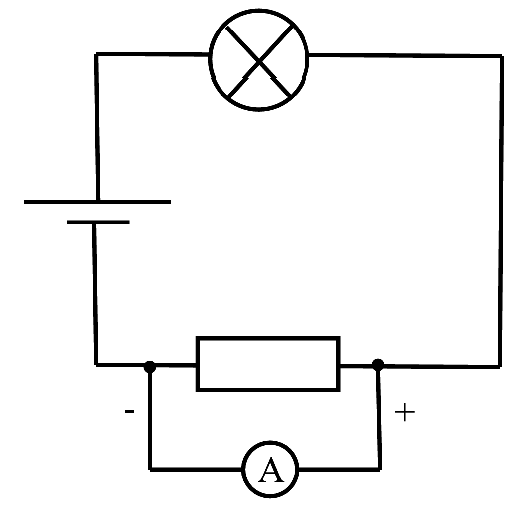
\includegraphics[width=0.4\columnwidth]{col11305.imgs/m38776_circuit1.png} % m38776;circuit1.png;;;6.0;8.5;
      \vspace{2pt}
    \vspace{.1in}
    \end{center}
 \end{figure}                
\label{m38776*uid90}\item (SC 2003/11) The emf of a battery can best be explained as the $\cdots $\label{m38776*id68404}\begin{enumerate}[noitemsep, label=\textbf{\alph*}. ] 
            \label{m38776*uid91}\item rate of energy delivered per unit current
\label{m38776*uid92}\item rate at which charge is delivered
\label{m38776*uid93}\item rate at which energy is delivered
\label{m38776*uid94}\item charge per unit of energy delivered by the battery
\end{enumerate}
                  \label{m38776*uid95}\item (IEB 2002/11 HG1) Which of the following is the correct definition of the emf of a battery?
\label{m38776*id68470}\begin{enumerate}[noitemsep, label=\textbf{\alph*}. ] 
            \label{m38776*uid96}\item It is the product of current and the external resistance of the circuit.
\label{m38776*uid97}\item It is a measure of the cell's ability to conduct an electric current.
\label{m38776*uid98}\item It is equal to the ``lost volts'' in the internal resistance of the circuit.
\label{m38776*uid99}\item It is the power supplied by the battery per unit current passing through the battery.
\end{enumerate}
                  \label{m38776*uid100}\item (IEB 2005/11 HG) Three identical light bulbs A, B and C are connected in an electric circuit as shown in the diagram below.
    \setcounter{subfigure}{0}
	\begin{figure}[H] % horizontal\label{m38776*id68542}
    \begin{center}
    \label{m38776*id68542!!!underscore!!!media}\label{m38776*id68542!!!underscore!!!printimage}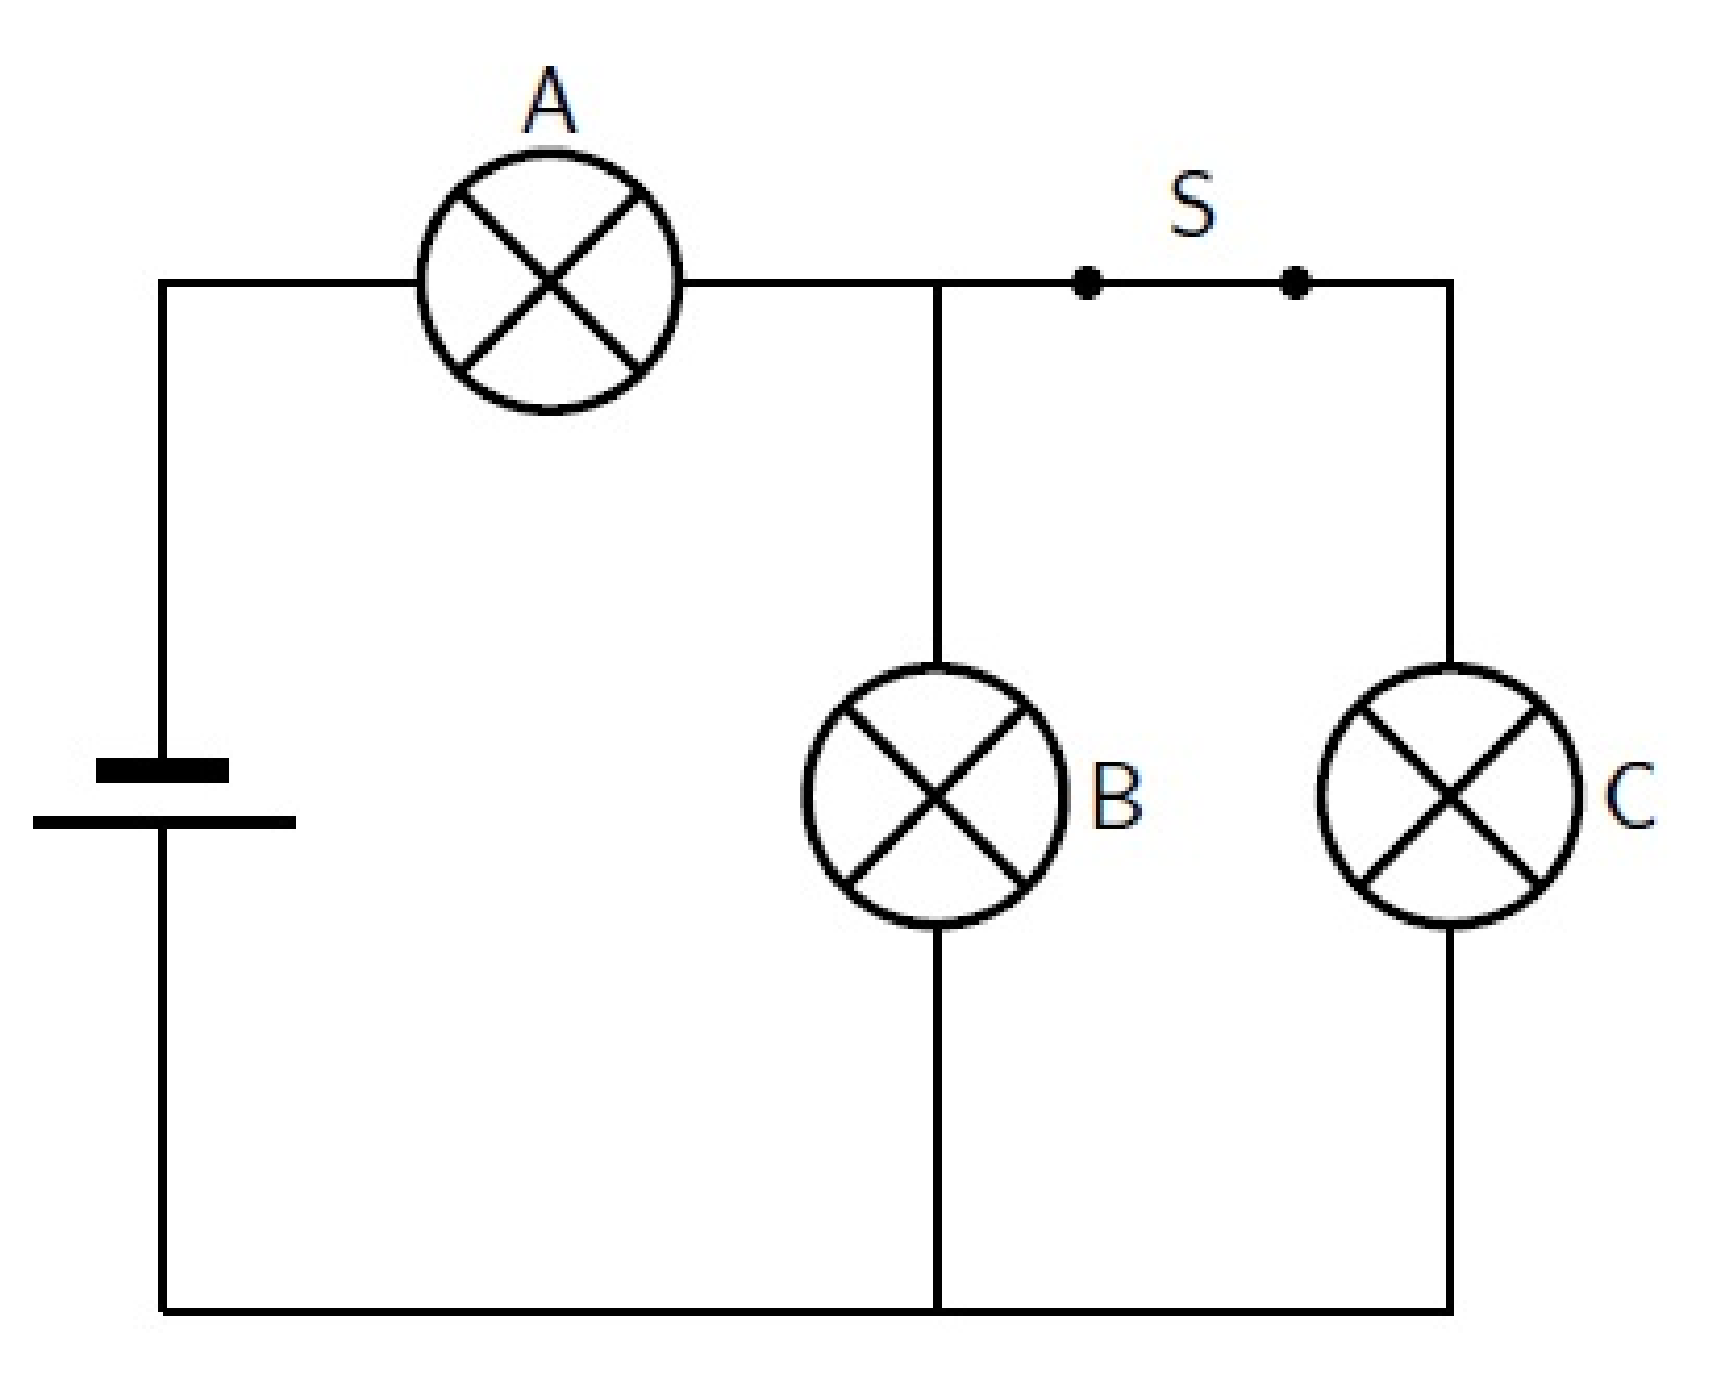
\includegraphics[width=300px]{col11305.imgs/m38776_PG10C9_037.png} % m38776;PG10C9\_037.png;;;6.0;8.5;
      \vspace{2pt}
    \vspace{.1in}
    \end{center}
 \end{figure}       \label{m38776*id68549}\begin{enumerate}[noitemsep, label=\textbf{\alph*}. ] 
            \label{m38776*uid101}\item How bright is bulb A compared to B and C?
\label{m38776*uid102}\item How bright are the bulbs after switch S has been opened?
\label{m38776*uid103}\item How do the currents in bulbs A and B change when switch S is opened?
    % \textbf{m38776*id68590}\par
          \begin{table}[H]
    % \begin{table}[H]
    % \\ 'id2959512' '1'
        \begin{center}
      \label{m38776*id68590}
    \noindent
    \tabletail{%
        \hline
        \multicolumn{3}{|p{\mytableboxwidth}|}{\raggedleft \small \sl continued on next page}\\
        \hline
      }
      \tablelasttail{}
      \begin{xtabular}[t]{|l|l|l|}\hline
         &
        \textbf{Current in A} &
        \textbf{Current in B}% make-rowspan-placeholders
     \tabularnewline\cline{1-1}\cline{2-2}\cline{3-3}
      %--------------------------------------------------------------------
        (a) &
        decreases &
        increases% make-rowspan-placeholders
     \tabularnewline\cline{1-1}\cline{2-2}\cline{3-3}
      %--------------------------------------------------------------------
        (b) &
        decreases &
        decreases% make-rowspan-placeholders
     \tabularnewline\cline{1-1}\cline{2-2}\cline{3-3}
      %--------------------------------------------------------------------
        (c) &
        increases &
        increases% make-rowspan-placeholders
     \tabularnewline\cline{1-1}\cline{2-2}\cline{3-3}
      %--------------------------------------------------------------------
        (d) &
        increases &
        decreases% make-rowspan-placeholders
     \tabularnewline\cline{1-1}\cline{2-2}\cline{3-3}
      %--------------------------------------------------------------------
    \end{xtabular}
      \end{center}
    \begin{center}{\small\bfseries Table 16.4}\end{center}
    \begin{caption}{\small\bfseries Table 16.4}\end{caption}
\end{table}
    \par
  \end{enumerate}
                  \label{m38776*uid104}\item (IEB 2004/11 HG1) When a current $I$ is maintained in a conductor for a time of $t$, how many electrons with charge e pass any cross-section of the conductor per second?
\label{m38776*id68784}\begin{enumerate}[noitemsep, label=\textbf{\alph*}. ] 
            \label{m38776*uid105}\item It
\label{m38776*uid106}\item It/e
\label{m38776*uid107}\item Ite
\label{m38776*uid108}\item e/It
\end{enumerate}
                  \end{enumerate}
  \label{m38776**end}
  \label{f13bac5321b85aca0e213ebdf4f72465**end}
\par \raisebox{-5 pt}{
\includegraphics[width=0.5cm]{col11305.imgs/summary_www.png}} Find the answers with the shortcodes:
 \par \begin{tabular}[h]{cccccc}
 (1.) lqX  &  (2.) lqI  &  (3.) lq5  &  (4.) lTw  &  (5.) lTv  &  (6.) lqn  &  (7.) lqR  &  (8.) lqN  &  (9.) lqQ  & \end{tabular}
